% +------------------------------------------------------------------------+
% | Reference manual page: Largest_empty_iso_rectangle_2.tex
% +------------------------------------------------------------------------+
% | 27.3.2000   Eli Packer
% | Package: 
% | 
%\RCSdef{\RCSTriangulationRev}{$Revision$}
%\RCSdefDate{\RCSTriangulationDate}{$Date$}
% |
%%RefPage: end of header, begin of main body
% +------------------------------------------------------------------------+


\begin{ccRefClass}{Largest_empty_iso_rectangle_2<T>}

%% \ccHtmlCrossLink{}     %% add further rules for cross referencing links
%% \ccHtmlIndexC[class]{} %% add further index entries

\begin{figure}[h]
\begin{ccTexOnly}
    \centerline{
      \includegraphics{ler_example.ps}
    }
\end{ccTexOnly}

\caption{An example of the largest empty iso rectangle of a set of points
\label{LER:example_pic}}

\begin{ccHtmlOnly}
    <P>
    <center>
        <img src="ler_example.gif"  border=0 alt="example output">
        <!--An example of the largest empty iso rectangle of a set of points-->
    </center>
\end{ccHtmlOnly}
\end{figure}

\ccDefinition
  
Given a set of points in the plane, the class \ccRefName\ is a data
structure that maintains an iso-rectangle with the largest area among
all iso-rectangles that are inside a given bounding box( iso-rectangle), and
that do not contain any point of the point set.

The class \ccRefName\ expects a model of the concept \ccc{LargestEmptyIsoRectangleTraits_2} as its template argument.  

\ccInclude{CGAL/Largest_empty_iso_rectangle_2.h}


\ccTypes
The class \ccClassTemplateName\ defines the following types:

\ccThreeToTwo

\ccTypedef{typedef T Traits;}{}

\ccTypedef{typedef Traits::Point_2 Point_2;}{}
\ccGlue
\ccTypedef{typedef Traits::Iso_rectangle_2 Iso_rectangle_2;}{}


The following iterator allows to enumerate the points. 
It is non mutable, bidirectional
and its value type is \ccc{Point_2}. 
It is invalidated by any insertion or removal of a point. 

\ccNestedType{const_iterator}{Iterator over the points.}


\ccCreation
\ccCreationVariable{l}  %% choose variable name
\ccSetTwoColumns{Qt_widget}{}
%\ccThree{Largest_empty_iso_rectangle_2<Traits>(const Point_2& bl, const Point_2& tr)}{}{}

\ccConstructor{Largest_empty_iso_rectangle_2<Traits>
(const Iso_rectangle_2 &b);}
{Constructor. The iso-rectangle \ccc{b} is the bounding rectangle.} 

\ccConstructor{Largest_empty_iso_rectangle_2<Traits>
(const Point_2 p,const Point_2 q);}
{Constructor. The iso-rectangle whose lower left and upper right points are \ccc{p} and
\ccc{q} respectively is the bounding rectangle.} 

\ccConstructor{Largest_empty_iso_rectangle_2<Traits>
();}
{Constructor. The iso-rectangle whose lower left point and upper right points are (0,0) 
and (1,1) respectively is the bounding rectangle.} 

\ccConstructor{Largest_empty_iso_rectangle_2<Traits>
(const Largest_empty_iso_rectangle_2<Traits> tr);}
{Copy constructor.} 

\ccConstructor{void ~Largest_empty_iso_rectangle_2<Traits>();}
{Destructor.}

\ccOperations
\ccSetThreeColumns{const_iterator}{container.begin() const;}{}

\ccHeading{Assignment}

\ccMethod{Largest_empty_iso_rectangle_2<Traits>
	operator=(const Largest_empty_iso_rectangle_2<Traits> & tr);}
{}



\ccAccessFunctions

\ccMethod{const Traits & traits() const;}
{Returns a const reference to the traits object.}


\ccMethod{const_iterator begin() const;}
{Returns an iterator to the beginning of the point set.}
\ccMethod{const_iterator end() const;}
{Returns a past-the-end iterator for the point set.}


\ccHeading{Queries}

\ccMethod{Quadruple<Point_2, Point_2, Point_2, Point_2>
  get_left_bottom_right_top();}
{Returns the four points that define the largest empty iso-rectangle.
Note that these points are almost never on a corner of an iso-rectangle.}
\ccGlue
\ccMethod{Iso_rectangle_2  get_largest_empty_iso_rectangle();}
{Returns the largest empty iso-rectangle. Note that the two
points defining the iso-rectangle are almost never part of 
the point set.}
\ccGlue
\ccMethod{Iso_rectangle_2 get_bounding_box();}
{Returns  the iso-rectangle passed in the constructor.}
\ccHeading{Insertion}


\ccMethod{void 
  insert(const Point_2& p);}
{Inserts point \ccc{p} in the point set, if it is not already in the set.}

\ccMethod{void 
  push_back(const Point_2& p);}
{Inserts point \ccc{p} in the point set, if it is not already in the set.}


\ccMethod{template < class InputIterator >
          int
          insert(InputIterator first, InputIterator last);}
{Inserts the points in the range $\left[\right.$\ccc{first},
\ccc{last}$\left.\right)$.  Returns the number of inserted points. \\ \\
\ccRequirements The \ccc{value_type} of \ccc{first} and \ccc{last} is \ccc{Point}.}

\ccHeading{Removal}

\ccMethod{bool remove(const Point_2& p);}{Removes point \ccc{p}.
Returns false iff \ccc{p} is not in the point set. }

\ccMethod{void clear();}
{Removes all points of \ccVar.}

%\ccSeeAlso

\ccImplementation

The algorithm is an implementation of \cite{o-naler-90}. The runtime of an
insertion or a removal is $O(\log n)$. A query takes $O(n^2)$ worst
case time and $O(n \log n)$ expected time. The working storage is $
O(n)$.







%\ccExample

%%\ccIncludeExampleCode{examples/Triangulation3/example1.C}

\bibliography{Largest_empty_iso_rectangle_2}
\bibliographystyle{abbrv}

\end{ccRefClass}

% +------------------------------------------------------------------------+
%%RefPage: end of main body, begin of footer
% EOF
% +------------------------------------------------------------------------+

